\section{Datenmodellierung}
MongoDB ist eine dokumentorientierte Datenbank. Dabei werden die Daten in JSON
ähnlichen Dokumenten verwaltet. Das bedeutet, dass die Daten nicht relational
verwaltet werden. So kann zum Beispiel in Tupel einer relationalen Datenbank
als Dokument in der dokumentorienterten Datenbank abgebildet werden. Die
Attribute und die dazugehörigen Werte werden dabei in Schlüssel-Wert Paare
abgebildet. 

 Unserem Projekt liegt das ER-Schema aus \ref{fig:uni-db}
zugrunde.
Da MongoDB eine NoSQL und keine relationale Datenbank ist, kann das ER-Schema nicht direkt
in dieser Form in der Datenbank abgebildet werden. 

\begin{figure}[h] 
	\centering
		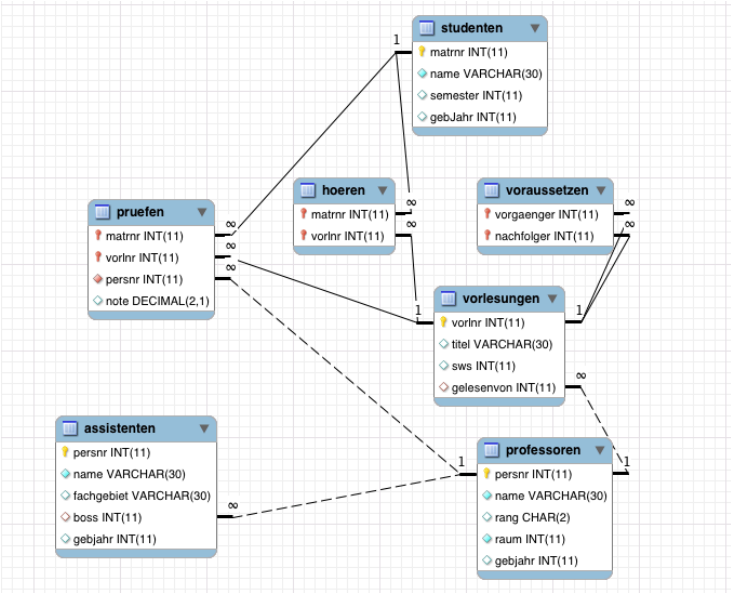
\includegraphics[width=1\textwidth]{./pictures/SQL-DB_ER_Diagramm_UNI-DB.png}
	\caption{ER-Diagramm zur Uni-DB \cite{Kaufmann2016}}
	\label{fig:uni-db}
\end{figure}

Eine Komposition bedeutet, dass z.B in der NoSQL Datenbank als ``teil von''
abgebildet wird. Eine Aggregation bedeutet, dass diese in Beziehung  als
Referenz abgebildet wird.

Im ER-Diagramm wird zum Beispiel die Komplex-Komplexe-Beziehung zwischen 
Vorlesungen und Studenten als eigene Tabelle abgebildet. In unserer Datenbank
wird diese Beziehung in zwei einfach-komplexe Beziehung abgebildet. Somit
besitzen Studenten eine Einfach-Komplexe Beziehung zu den Vorlesungen.
Diese Beziehung wird im JSON -Format im Feld Hören ersichtlich. Die vom
Studenten besuchten Vorlesungen werden als Vorlesungsnummer in einem Array
referenziert.
\begin{figure}
	\begin{verbatim}
	{
		"Legi": 25403,
		"Name" : "Jonas",
		"Semester" : 12,
		"Hören" : [5032, 1910],
	}
	\end{verbatim}
	\label{cod:vorlesung}
\end{figure}



